%-*- Mode:LaTeX; -*-      
\documentclass[11pt]{article}
\usepackage{vmargin}		% Force narrower margins
\usepackage{tikz-qtree}
\usepackage{tikz-dependency}
\setpapersize{USletter}
\setmarginsrb{1.0in}{1.0in}{1.0in}{0.6in}{0pt}{0pt}{0pt}{0.4in}
\setlength{\parskip}{.1in}  % removed space between paragraphs
\setlength{\parindent}{0in}
\usepackage{amsmath}
\usepackage{tabu}
\usepackage{epsfig}
\usepackage{graphicx}
\newcommand{\ra}{$\rightarrow$~}
\newcommand{\dt}{$\circ$~}

\begin{document}

\large
\begin{center}
{\bf CS-5340/6340, Written Assignment \#2} \\
{\bf DUE: Thursday September 20, 2018 by 11:59pm}
\end{center}
\normalsize

\begin{enumerate}  



\item (24 pts)
\begin{enumerate} 

\item Suppose a shallow parser (chunker) is applied to the sentences
  below. Label all prepositional phrase (PP) chunks and base noun
  phrase (NP) chunks that should be produced for each sentence. Be sure
  to label an NP even if it is nested in a PP. For examples {\it `He stays
  in Salt Lake City'} should be `[NP: He] stays [PP: in [NP: Salt Lake
  City]]'. \\

\begin{enumerate}

\item John gave Mary a book as a gift.  	 
\vspace*{.3in}

\item A person in the park threw a bone to his dog.
\vspace*{.3in}

\item In July Bob will sell his food truck.
\vspace*{.3in} 

\item The mouse the cat caught died.
\vspace*{.3in}

\item The storm destroyed a large number of properties in the city. 
\vspace*{.3in}


\end{enumerate}
\item Label each sentence below with BIO tags corresponding to the NP
  chunks that you identified in part (a). \\


\begin{enumerate}

\item John gave Mary a book as a gift.  	
 
\vspace*{.3in}


\item A person in the park threw a bone to his dog.

\vspace*{.3in}


\item In July Bob will sell his food truck.

\vspace*{.3in} 

\item The mouse the cat caught died.

\vspace*{.3in}

\item The storm destroyed a large number of properties in the city.
 
\vspace*{.3in}


\end{enumerate}

\end{enumerate}


\newpage
\item (24 pts) In this question, you are going to use the CKY
  algorithm to parse a sentence. (Use the ordinary CKY algorithm, \underline{not}
 probabilistic CKY.)
\begin{enumerate}


\item List all table entries  produced by the CKY algorithm for
  the sentence {\it `John eats the steak with chopsticks'} using the grammar
  below. Each entry table[i,j] refers to the cell  for row i and
  column j in the table. For example, table[1,4] should contain constituents that span words 1
  through 4.\\

\fbox{\parbox{0.4\textwidth}{
S \ra NP VP\\
NP \ra NP PP \\
NP \ra art noun \\
PP \ra prep NP \\
VP \ra VP PP  \\
VP \ra verb NP\\
\\
NP \ra John \\
NP \ra chopsticks \\
NP \ra steak \\
noun \ra John \\
noun \ra chopsticks \\
noun \ra steak \\
verb \ra eats \\
prep \ra with \\
art \ra the


}
}
\\\\\\

\textbf{table[1,1]}: \\
\textbf{table[1,2]}: \\
\textbf{table[1,3]}: \\
\textbf{table[1,4]}: \\
\textbf{table[1,5]}: \\
\textbf{table[1,6]}: \\
\textbf{table[2,2]}: \\
\textbf{table[2,3]}: \\
\textbf{table[2,4]}: \\
\textbf{table[2,5]}: \\
\textbf{table[2,6]}: \\
\textbf{table[3,3]}: \\
\textbf{table[3,4]}: \\
\textbf{table[3,5]}: \\
\textbf{table[3,6]}: \\
\textbf{table[4,4]}: \\
\textbf{table[4,5]}: \\
\textbf{table[4,6]}: \\
\textbf{table[5,5]}: \\
\textbf{table[5,6]}: \\
\textbf{table[6,6]}: \\


\newpage

\item Draw the parse tree for every S constituent produced in the
  table for part (a). For each one, please indicate which cell the S constituent appears in.

\vspace{3in}


\end{enumerate}


\newpage

\item (18 Pts) Given the grammar G2 and the sentence {\it `the dog park is
  closed'}, fill in a chart using the Earley chart parsing
  algorithm. Each chart entry should be a constituent or a rule, with
  a start and end position indicating the range of words that have
  been matched by the constituent or rule. For example, `NP[1-4]'
  should be used for an NP that matches words in positions 1-3 (thus ends at
  position 4). Similarly, `S \ra NP * VP
  [1,3]' means that the NP has matched the words in positions
  1-2 and the rule is  anticipating a VP starting in position
  3. Assume that the first word in the   sentence is in position 1.

\begin{center}
\begin{tabular}{|l|} \hline 
\textbf{G2}  \\  
S \ra NP VP    \\
S \ra VP NP     \\
VP \ra verb VP     \\
VP \ra verb \\
NP \ra art NP    \\
NP \ra noun noun \\  \\
noun \ra dog $\mid$ park \\
verb \ra closed $\mid$ park $\mid$ is \\
art \ra the \\
\hline
\end{tabular}\end{center}

Below, we have created the part-of-speech constituents that belong in the chart to get you
started. Please fill in the remaining entries!

\begin{center}
 \begin{tabular}{lc} {\bf Constituent or Rule~~~} & {\bf ~~~Start-End} \\ \hline 
 art(``the'') &  [1-2] \\
 noun(``dog'') & [2-3] \\
 noun(``park'') & [3-4] \\
 verb(``park'') & [3-4]  \\
 verb(``is'') & [4-5] \\
 verb(``closed'') & [5-6]\\\hline\\
 add your entries here ...  & ...\\
 add your entries here ... &  ...\\
 add your entries here ... & ...\\ 
\end{tabular}\end{center}



\newpage
\item (14 pts) Consider the four parse trees below:

\begin{figure}[h]
\begin{minipage}[b]{0.5\linewidth}
\centering
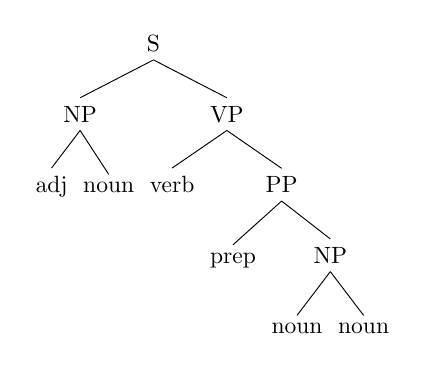
\begin{tikzpicture}[scale=.85, sibling distance=0pt]

\Tree [.S  [.NP adj noun ] 
           [.VP verb [.PP prep 
                              [.NP noun noun ] 
                     ] 
           ] 
      ]
\end{tikzpicture}
\end{minipage}
\begin{minipage}[b]{0.5\linewidth}
\centering
\begin{tikzpicture}[scale=.85, sibling distance=0pt]

\Tree [.S  [ .VP verb [.NP [adj noun ] ][ [.PP [prep [.NP art [.NP adj noun ] ] ] ]] ] 
                  ]
\end{tikzpicture}
\end{minipage}
\end{figure}

\begin{figure}[h]	
\begin{minipage}[b]{0.5\linewidth}
\centering
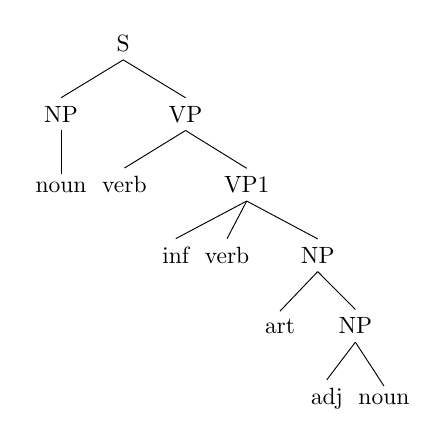
\begin{tikzpicture}[scale=.85, sibling distance=0pt]    

\Tree [.S [.NP noun ] 
		  [.VP  verb 
			[.VP1 inf verb 
				[.NP art [.NP adj noun ] 
				] 
			]		  
		  ]          
      ]
\end{tikzpicture}
\end{minipage}
\begin{minipage}[b]{0.5\linewidth}
\centering
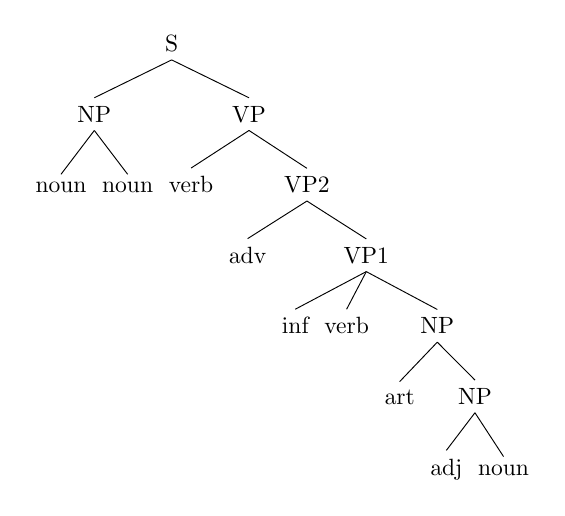
\begin{tikzpicture}[scale=.85, sibling distance=0pt]   

\Tree [.S [.NP noun noun ] 
  		  [.VP verb 
  		  	   [.VP2 adv [.VP1 inf verb 
  		  	                 [.NP art 
  		  	                           [.NP adj noun ]
  		  	                  ] 
  		                ] 
  	            ]
  	       ]
  	  ]
\end{tikzpicture}
\end{minipage}
\end{figure}

Consider these four parse trees to be a (tiny!) Treebank, and construct a
probabilistic context-free grammar (PCFG) from this Treebank. 
List all distinct context-free grammar rules that are depicted in the
trees above and compute their probabilities.

\begin{center}
	\begin{tabular}{l@{\hskip 1in}c} 
	 \textbf{Rules~~~~~~~~~~~~~~~} & \textbf{Probability~~~~~~~~~~~~~~~~~} \\ \hline 
 \end{tabular}
\end{center}



\newpage
\item (20 pts) For each sentence below, draw the dependency relations
  that would be produced by applying the given sequence of
  shift-reduce operations. w$_{i}$ means the i$^{th}$ word in the
  sentence. (The dependency relations will be {\it unlabeled} directed
  edges.)
  \\
	%to draw a tree in latex, refer to the lines for trees in part b) below
	
	\begin{enumerate}
		\item
		SENTENCE: w$_{1}$ w$_{2}$ w$_{3}$ w$_{4}$ w$_{5}$ w$_{6}$ \\\\
		OPERATIONS: Shift, Shift, LeftArc, Shift, Shift, RightArc, RightArc, Shift, Shift, LeftArc, RightArc \\

		\vspace{.5in}
	
	
	
		\item
		SENTENCE: w$_{1}$ w$_{2}$ w$_{3}$ w$_{4}$ w$_{5}$ w$_{6}$ w$_{7}$ \\
		
		OPERATIONS: Shift, Shift, LeftArc, Shift, Shift, LeftArc, Shift, Shift, Shift, LeftArc, LeftArc, RightArc, RightArc\\

		\vspace{.5in}
	\end{enumerate}

\newpage

\underline{\textbf{Question \#6 is for CS-6340 students ONLY!}}  \\

\item	(13 pts) For each dependency graph below, 
        determine the sequence of shift-reduce operations that should be
        predicted by the oracle in order to produce the graph.\\ 

	% lines for dependency tree 
	\vspace{0.5in}
	\begin{dependency}[edge slant=15pt,label theme = simple, edge theme = iron]
  		\begin{deptext}[column sep=1em]
    			The \& apple \&  eaten \& by \& John \& was \& rotten\\ \\ \\
  		\end{deptext}
  		\depedge{2}{1}{}
  		\depedge{2}{3}{}  
  		\depedge{7}{2}{}
  		\depedge{7}{6}{}
  		\depedge{3}{5}{}
  		\depedge{5}{4}{}

		\end{dependency}

	\vspace{.5in}


	\begin{dependency}[edge slant=15pt,label theme = simple, edge theme = iron]
  	\begin{deptext}[column sep=1em]
    		This \& year \& they \& are \& moving \& even \& faster \\ \\ \\
  	\end{deptext}
  	\depedge{2}{1}{}
  	\depedge{5}{3}{}
  	\depedge{5}{4}{}
  	\depedge{5}{2}{}
  	\depedge{5}{7}{}
  	\depedge{7}{6}{}
	\end{dependency}
	
	\vspace{1in}
	

\end{enumerate}  % END OF WRITTEN QUESTIONS


\newpage
\hspace*{1.5in}  {\bf ELECTRONIC SUBMISSION INSTRUCTIONS} \\

You should submit the answers to this assignment {\bf in pdf format}
on our course's CANVAS site by 11:59pm on Thursday, September 20.

\end{document}


